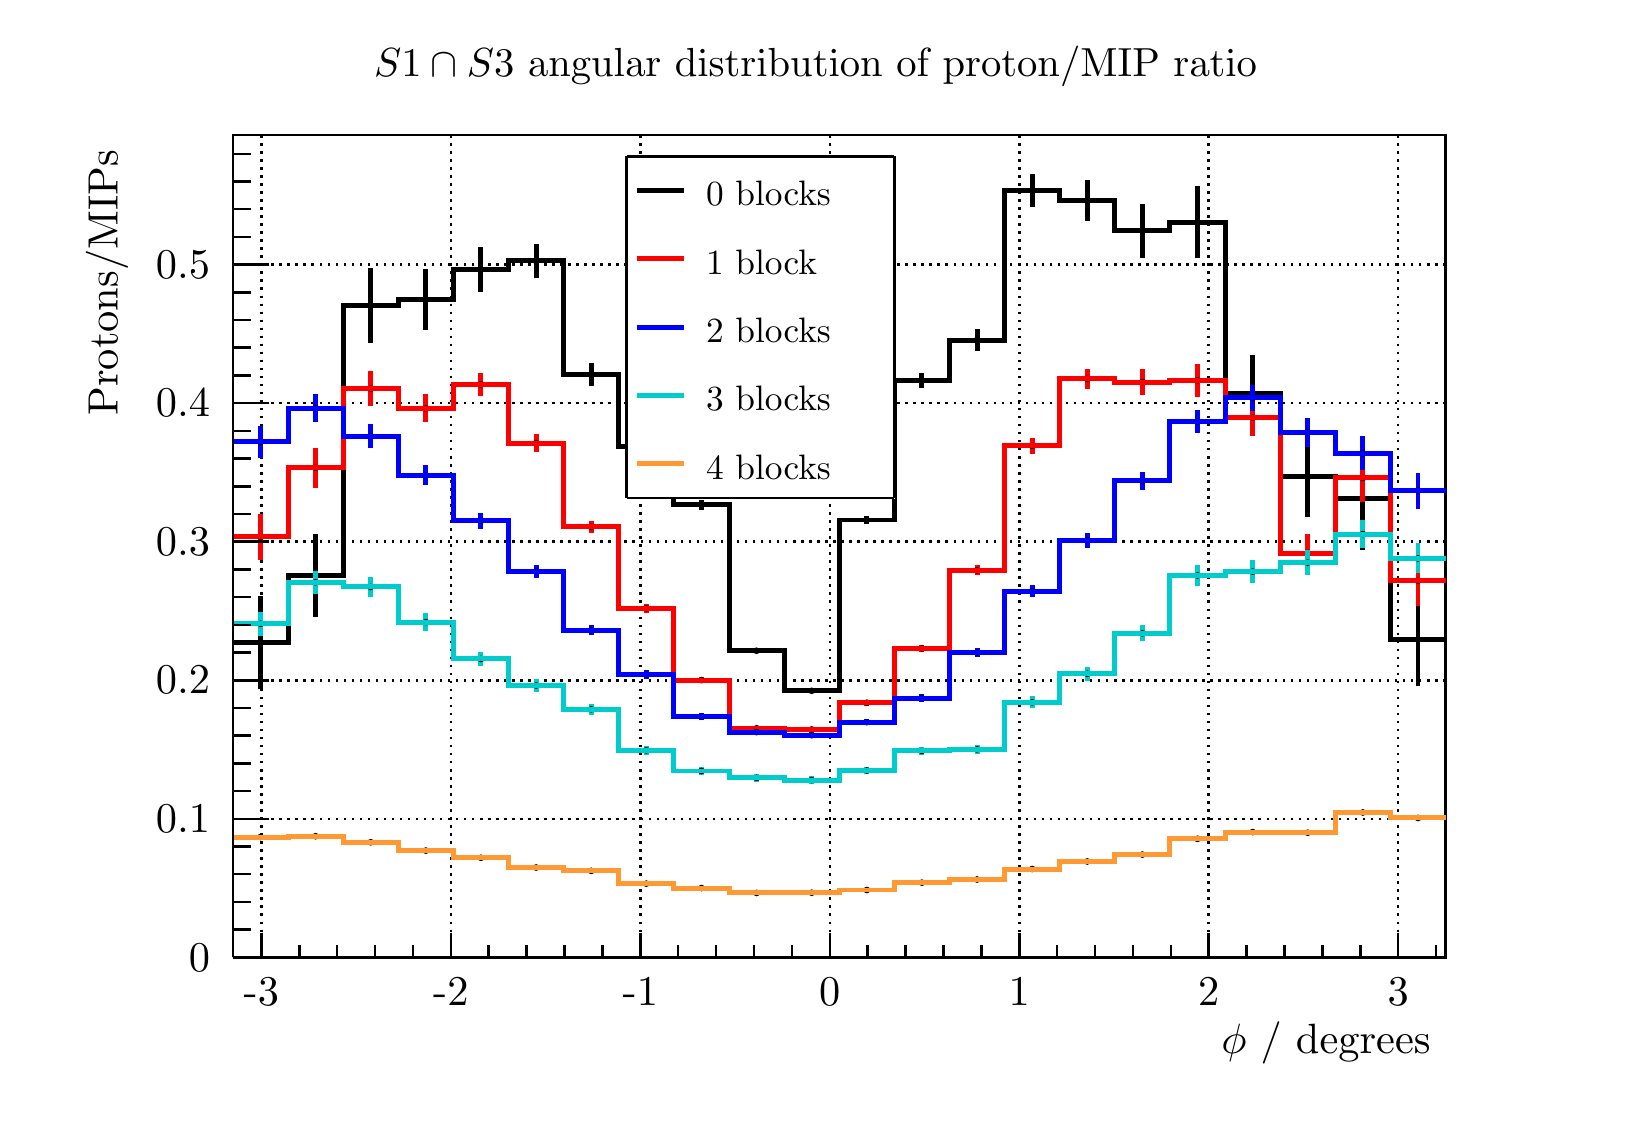
\begin{tikzpicture}
\pgfdeclareplotmark{cross} {
\pgfpathmoveto{\pgfpoint{-0.3\pgfplotmarksize}{\pgfplotmarksize}}
\pgfpathlineto{\pgfpoint{+0.3\pgfplotmarksize}{\pgfplotmarksize}}
\pgfpathlineto{\pgfpoint{+0.3\pgfplotmarksize}{0.3\pgfplotmarksize}}
\pgfpathlineto{\pgfpoint{+1\pgfplotmarksize}{0.3\pgfplotmarksize}}
\pgfpathlineto{\pgfpoint{+1\pgfplotmarksize}{-0.3\pgfplotmarksize}}
\pgfpathlineto{\pgfpoint{+0.3\pgfplotmarksize}{-0.3\pgfplotmarksize}}
\pgfpathlineto{\pgfpoint{+0.3\pgfplotmarksize}{-1.\pgfplotmarksize}}
\pgfpathlineto{\pgfpoint{-0.3\pgfplotmarksize}{-1.\pgfplotmarksize}}
\pgfpathlineto{\pgfpoint{-0.3\pgfplotmarksize}{-0.3\pgfplotmarksize}}
\pgfpathlineto{\pgfpoint{-1.\pgfplotmarksize}{-0.3\pgfplotmarksize}}
\pgfpathlineto{\pgfpoint{-1.\pgfplotmarksize}{0.3\pgfplotmarksize}}
\pgfpathlineto{\pgfpoint{-0.3\pgfplotmarksize}{0.3\pgfplotmarksize}}
\pgfpathclose
\pgfusepathqstroke
}
\pgfdeclareplotmark{cross*} {
\pgfpathmoveto{\pgfpoint{-0.3\pgfplotmarksize}{\pgfplotmarksize}}
\pgfpathlineto{\pgfpoint{+0.3\pgfplotmarksize}{\pgfplotmarksize}}
\pgfpathlineto{\pgfpoint{+0.3\pgfplotmarksize}{0.3\pgfplotmarksize}}
\pgfpathlineto{\pgfpoint{+1\pgfplotmarksize}{0.3\pgfplotmarksize}}
\pgfpathlineto{\pgfpoint{+1\pgfplotmarksize}{-0.3\pgfplotmarksize}}
\pgfpathlineto{\pgfpoint{+0.3\pgfplotmarksize}{-0.3\pgfplotmarksize}}
\pgfpathlineto{\pgfpoint{+0.3\pgfplotmarksize}{-1.\pgfplotmarksize}}
\pgfpathlineto{\pgfpoint{-0.3\pgfplotmarksize}{-1.\pgfplotmarksize}}
\pgfpathlineto{\pgfpoint{-0.3\pgfplotmarksize}{-0.3\pgfplotmarksize}}
\pgfpathlineto{\pgfpoint{-1.\pgfplotmarksize}{-0.3\pgfplotmarksize}}
\pgfpathlineto{\pgfpoint{-1.\pgfplotmarksize}{0.3\pgfplotmarksize}}
\pgfpathlineto{\pgfpoint{-0.3\pgfplotmarksize}{0.3\pgfplotmarksize}}
\pgfpathclose
\pgfusepathqfillstroke
}
\pgfdeclareplotmark{newstar} {
\pgfpathmoveto{\pgfqpoint{0pt}{\pgfplotmarksize}}
\pgfpathlineto{\pgfqpointpolar{44}{0.5\pgfplotmarksize}}
\pgfpathlineto{\pgfqpointpolar{18}{\pgfplotmarksize}}
\pgfpathlineto{\pgfqpointpolar{-20}{0.5\pgfplotmarksize}}
\pgfpathlineto{\pgfqpointpolar{-54}{\pgfplotmarksize}}
\pgfpathlineto{\pgfqpointpolar{-90}{0.5\pgfplotmarksize}}
\pgfpathlineto{\pgfqpointpolar{234}{\pgfplotmarksize}}
\pgfpathlineto{\pgfqpointpolar{198}{0.5\pgfplotmarksize}}
\pgfpathlineto{\pgfqpointpolar{162}{\pgfplotmarksize}}
\pgfpathlineto{\pgfqpointpolar{134}{0.5\pgfplotmarksize}}
\pgfpathclose
\pgfusepathqstroke
}
\pgfdeclareplotmark{newstar*} {
\pgfpathmoveto{\pgfqpoint{0pt}{\pgfplotmarksize}}
\pgfpathlineto{\pgfqpointpolar{44}{0.5\pgfplotmarksize}}
\pgfpathlineto{\pgfqpointpolar{18}{\pgfplotmarksize}}
\pgfpathlineto{\pgfqpointpolar{-20}{0.5\pgfplotmarksize}}
\pgfpathlineto{\pgfqpointpolar{-54}{\pgfplotmarksize}}
\pgfpathlineto{\pgfqpointpolar{-90}{0.5\pgfplotmarksize}}
\pgfpathlineto{\pgfqpointpolar{234}{\pgfplotmarksize}}
\pgfpathlineto{\pgfqpointpolar{198}{0.5\pgfplotmarksize}}
\pgfpathlineto{\pgfqpointpolar{162}{\pgfplotmarksize}}
\pgfpathlineto{\pgfqpointpolar{134}{0.5\pgfplotmarksize}}
\pgfpathclose
\pgfusepathqfillstroke
}
\definecolor{c}{rgb}{1,1,1};
\draw [color=c, fill=c] (0,0) rectangle (20,13.5632);
\draw [color=c, fill=c] (2.6,1.76322) rectangle (18,12.2069);
\definecolor{c}{rgb}{0,0,0};
\draw [c,line width=0.9] (2.6,1.76322) -- (2.6,12.2069) -- (18,12.2069) -- (18,1.76322) -- (2.6,1.76322);
\definecolor{c}{rgb}{1,1,1};
\draw [color=c, fill=c] (2.6,1.76322) rectangle (18,12.2069);
\definecolor{c}{rgb}{0,0,0};
\draw [c,line width=0.9] (2.6,1.76322) -- (2.6,12.2069) -- (18,12.2069) -- (18,1.76322) -- (2.6,1.76322);
\draw [c,line width=0.9] (2.6,1.76322) -- (18,1.76322);
\draw [c,dotted,line width=0.9] (2.96094,12.2069) -- (2.96094,1.76322);
\draw [c,dotted,line width=0.9] (5.36719,12.2069) -- (5.36719,1.76322);
\draw [c,dotted,line width=0.9] (7.77344,12.2069) -- (7.77344,1.76322);
\draw [c,dotted,line width=0.9] (10.1797,12.2069) -- (10.1797,1.76322);
\draw [c,dotted,line width=0.9] (12.5859,12.2069) -- (12.5859,1.76322);
\draw [c,dotted,line width=0.9] (14.9922,12.2069) -- (14.9922,1.76322);
\draw [c,dotted,line width=0.9] (17.3984,12.2069) -- (17.3984,1.76322);
\draw [c,dotted,line width=0.9] (2.96094,12.2069) -- (2.96094,1.76322);
\draw [c,dotted,line width=0.9] (17.3984,12.2069) -- (17.3984,1.76322);
\draw [c,line width=0.9] (2.6,1.76322) -- (2.6,12.2069);
\draw [c,dotted,line width=0.9] (18,1.76322) -- (2.6,1.76322);
\draw [c,dotted,line width=0.9] (18,3.52278) -- (2.6,3.52278);
\draw [c,dotted,line width=0.9] (18,5.28233) -- (2.6,5.28233);
\draw [c,dotted,line width=0.9] (18,7.04189) -- (2.6,7.04189);
\draw [c,dotted,line width=0.9] (18,8.80145) -- (2.6,8.80145);
\draw [c,dotted,line width=0.9] (18,10.561) -- (2.6,10.561);
\draw [c,dotted,line width=0.9] (18,10.561) -- (2.6,10.561);
\definecolor{c}{rgb}{0,0,0.6};
\draw [c,line width=0.9] (2.6,1.76322) -- (3.3,1.76322) -- (3.3,1.76322) -- (4,1.76322) -- (4,1.76322) -- (4.7,1.76322) -- (4.7,1.76322) -- (5.4,1.76322) -- (5.4,1.76322) -- (6.1,1.76322) -- (6.1,1.76322) -- (6.8,1.76322) -- (6.8,1.76322) --
 (7.5,1.76322) -- (7.5,1.76322) -- (8.2,1.76322) -- (8.2,1.76322) -- (8.9,1.76322) -- (8.9,1.76322) -- (9.6,1.76322) -- (9.6,1.76322) -- (10.3,1.76322) -- (10.3,1.76322) -- (11,1.76322) -- (11,1.76322) -- (11.7,1.76322) -- (11.7,1.76322) --
 (12.4,1.76322) -- (12.4,1.76322) -- (13.1,1.76322) -- (13.1,1.76322) -- (13.8,1.76322) -- (13.8,1.76322) -- (14.5,1.76322) -- (14.5,1.76322) -- (15.2,1.76322) -- (15.2,1.76322) -- (15.9,1.76322) -- (15.9,1.76322) -- (16.6,1.76322) -- (16.6,1.76322)
 -- (17.3,1.76322) -- (17.3,1.76322) -- (18,1.76322);
\definecolor{c}{rgb}{0,0,0};
\draw [c,line width=0.9] (2.6,1.76322) -- (18,1.76322);
\draw [anchor= east] (18,0.678161) node[scale=1.5317, color=c, rotate=0]{$\phi$ / degrees};
\draw [c,line width=0.9] (2.96094,2.07653) -- (2.96094,1.76322);
\draw [c,line width=0.9] (3.44219,1.91987) -- (3.44219,1.76322);
\draw [c,line width=0.9] (3.92344,1.91987) -- (3.92344,1.76322);
\draw [c,line width=0.9] (4.40469,1.91987) -- (4.40469,1.76322);
\draw [c,line width=0.9] (4.88594,1.91987) -- (4.88594,1.76322);
\draw [c,line width=0.9] (5.36719,2.07653) -- (5.36719,1.76322);
\draw [c,line width=0.9] (5.84844,1.91987) -- (5.84844,1.76322);
\draw [c,line width=0.9] (6.32969,1.91987) -- (6.32969,1.76322);
\draw [c,line width=0.9] (6.81094,1.91987) -- (6.81094,1.76322);
\draw [c,line width=0.9] (7.29219,1.91987) -- (7.29219,1.76322);
\draw [c,line width=0.9] (7.77344,2.07653) -- (7.77344,1.76322);
\draw [c,line width=0.9] (8.25469,1.91987) -- (8.25469,1.76322);
\draw [c,line width=0.9] (8.73594,1.91987) -- (8.73594,1.76322);
\draw [c,line width=0.9] (9.21719,1.91987) -- (9.21719,1.76322);
\draw [c,line width=0.9] (9.69844,1.91987) -- (9.69844,1.76322);
\draw [c,line width=0.9] (10.1797,2.07653) -- (10.1797,1.76322);
\draw [c,line width=0.9] (10.6609,1.91987) -- (10.6609,1.76322);
\draw [c,line width=0.9] (11.1422,1.91987) -- (11.1422,1.76322);
\draw [c,line width=0.9] (11.6234,1.91987) -- (11.6234,1.76322);
\draw [c,line width=0.9] (12.1047,1.91987) -- (12.1047,1.76322);
\draw [c,line width=0.9] (12.5859,2.07653) -- (12.5859,1.76322);
\draw [c,line width=0.9] (13.0672,1.91987) -- (13.0672,1.76322);
\draw [c,line width=0.9] (13.5484,1.91987) -- (13.5484,1.76322);
\draw [c,line width=0.9] (14.0297,1.91987) -- (14.0297,1.76322);
\draw [c,line width=0.9] (14.5109,1.91987) -- (14.5109,1.76322);
\draw [c,line width=0.9] (14.9922,2.07653) -- (14.9922,1.76322);
\draw [c,line width=0.9] (15.4734,1.91987) -- (15.4734,1.76322);
\draw [c,line width=0.9] (15.9547,1.91987) -- (15.9547,1.76322);
\draw [c,line width=0.9] (16.4359,1.91987) -- (16.4359,1.76322);
\draw [c,line width=0.9] (16.9172,1.91987) -- (16.9172,1.76322);
\draw [c,line width=0.9] (17.3984,2.07653) -- (17.3984,1.76322);
\draw [c,line width=0.9] (2.96094,2.07653) -- (2.96094,1.76322);
\draw [c,line width=0.9] (17.3984,2.07653) -- (17.3984,1.76322);
\draw [c,line width=0.9] (17.8797,1.91987) -- (17.8797,1.76322);
\draw [anchor=base] (2.96094,1.15287) node[scale=1.5317, color=c, rotate=0]{-3};
\draw [anchor=base] (5.36719,1.15287) node[scale=1.5317, color=c, rotate=0]{-2};
\draw [anchor=base] (7.77344,1.15287) node[scale=1.5317, color=c, rotate=0]{-1};
\draw [anchor=base] (10.1797,1.15287) node[scale=1.5317, color=c, rotate=0]{0};
\draw [anchor=base] (12.5859,1.15287) node[scale=1.5317, color=c, rotate=0]{1};
\draw [anchor=base] (14.9922,1.15287) node[scale=1.5317, color=c, rotate=0]{2};
\draw [anchor=base] (17.3984,1.15287) node[scale=1.5317, color=c, rotate=0]{3};
\draw [c,line width=0.9] (2.6,1.76322) -- (2.6,12.2069);
\draw [anchor= east] (1,12.2069) node[scale=1.5317, color=c, rotate=90]{  Protons/MIPs};
\draw [c,line width=0.9] (3.062,1.76322) -- (2.6,1.76322);
\draw [c,line width=0.9] (2.831,2.11513) -- (2.6,2.11513);
\draw [c,line width=0.9] (2.831,2.46704) -- (2.6,2.46704);
\draw [c,line width=0.9] (2.831,2.81895) -- (2.6,2.81895);
\draw [c,line width=0.9] (2.831,3.17086) -- (2.6,3.17086);
\draw [c,line width=0.9] (3.062,3.52278) -- (2.6,3.52278);
\draw [c,line width=0.9] (2.831,3.87469) -- (2.6,3.87469);
\draw [c,line width=0.9] (2.831,4.2266) -- (2.6,4.2266);
\draw [c,line width=0.9] (2.831,4.57851) -- (2.6,4.57851);
\draw [c,line width=0.9] (2.831,4.93042) -- (2.6,4.93042);
\draw [c,line width=0.9] (3.062,5.28233) -- (2.6,5.28233);
\draw [c,line width=0.9] (2.831,5.63425) -- (2.6,5.63425);
\draw [c,line width=0.9] (2.831,5.98616) -- (2.6,5.98616);
\draw [c,line width=0.9] (2.831,6.33807) -- (2.6,6.33807);
\draw [c,line width=0.9] (2.831,6.68998) -- (2.6,6.68998);
\draw [c,line width=0.9] (3.062,7.04189) -- (2.6,7.04189);
\draw [c,line width=0.9] (2.831,7.3938) -- (2.6,7.3938);
\draw [c,line width=0.9] (2.831,7.74572) -- (2.6,7.74572);
\draw [c,line width=0.9] (2.831,8.09763) -- (2.6,8.09763);
\draw [c,line width=0.9] (2.831,8.44954) -- (2.6,8.44954);
\draw [c,line width=0.9] (3.062,8.80145) -- (2.6,8.80145);
\draw [c,line width=0.9] (2.831,9.15336) -- (2.6,9.15336);
\draw [c,line width=0.9] (2.831,9.50527) -- (2.6,9.50527);
\draw [c,line width=0.9] (2.831,9.85719) -- (2.6,9.85719);
\draw [c,line width=0.9] (2.831,10.2091) -- (2.6,10.2091);
\draw [c,line width=0.9] (3.062,10.561) -- (2.6,10.561);
\draw [c,line width=0.9] (3.062,10.561) -- (2.6,10.561);
\draw [c,line width=0.9] (2.831,10.9129) -- (2.6,10.9129);
\draw [c,line width=0.9] (2.831,11.2648) -- (2.6,11.2648);
\draw [c,line width=0.9] (2.831,11.6167) -- (2.6,11.6167);
\draw [c,line width=0.9] (2.831,11.9687) -- (2.6,11.9687);
\draw [anchor= east] (2.5,1.76322) node[scale=1.5317, color=c, rotate=0]{0};
\draw [anchor= east] (2.5,3.52278) node[scale=1.5317, color=c, rotate=0]{0.1};
\draw [anchor= east] (2.5,5.28233) node[scale=1.5317, color=c, rotate=0]{0.2};
\draw [anchor= east] (2.5,7.04189) node[scale=1.5317, color=c, rotate=0]{0.3};
\draw [anchor= east] (2.5,8.80145) node[scale=1.5317, color=c, rotate=0]{0.4};
\draw [anchor= east] (2.5,10.561) node[scale=1.5317, color=c, rotate=0]{0.5};
\draw [c,line width=1.8] (2.95,5.16802) -- (2.95,5.76221);
\draw [c,line width=1.8] (2.95,5.76221) -- (2.95,6.35641);
\foreach \P in {(2.95,5.76221)}{\draw[mark options={color=c,fill=c},mark size=2.402402pt,mark=*,mark size=1pt] plot coordinates {\P};}
\draw [c,line width=1.8] (3.65,6.08767) -- (3.65,6.61178);
\draw [c,line width=1.8] (3.65,6.61178) -- (3.65,7.13589);
\foreach \P in {(3.65,6.61178)}{\draw[mark options={color=c,fill=c},mark size=2.402402pt,mark=*,mark size=1pt] plot coordinates {\P};}
\draw [c,line width=1.8] (4.35,9.56273) -- (4.35,10.0404);
\draw [c,line width=1.8] (4.35,10.0404) -- (4.35,10.5181);
\foreach \P in {(4.35,10.0404)}{\draw[mark options={color=c,fill=c},mark size=2.402402pt,mark=*,mark size=1pt] plot coordinates {\P};}
\draw [c,line width=1.8] (5.05,9.72594) -- (5.05,10.1142);
\draw [c,line width=1.8] (5.05,10.1142) -- (5.05,10.5026);
\foreach \P in {(5.05,10.1142)}{\draw[mark options={color=c,fill=c},mark size=2.402402pt,mark=*,mark size=1pt] plot coordinates {\P};}
\draw [c,line width=1.8] (5.75,10.2136) -- (5.75,10.4971);
\draw [c,line width=1.8] (5.75,10.4971) -- (5.75,10.7806);
\foreach \P in {(5.75,10.4971)}{\draw[mark options={color=c,fill=c},mark size=2.402402pt,mark=*,mark size=1pt] plot coordinates {\P};}
\draw [c,line width=1.8] (6.45,10.3922) -- (6.45,10.6092);
\draw [c,line width=1.8] (6.45,10.6092) -- (6.45,10.8262);
\foreach \P in {(6.45,10.6092)}{\draw[mark options={color=c,fill=c},mark size=2.402402pt,mark=*,mark size=1pt] plot coordinates {\P};}
\draw [c,line width=1.8] (7.15,9.01643) -- (7.15,9.16611);
\draw [c,line width=1.8] (7.15,9.16611) -- (7.15,9.31579);
\foreach \P in {(7.15,9.16611)}{\draw[mark options={color=c,fill=c},mark size=2.402402pt,mark=*,mark size=1pt] plot coordinates {\P};}
\draw [c,line width=1.8] (7.85,8.15111) -- (7.85,8.25348);
\draw [c,line width=1.8] (7.85,8.25348) -- (7.85,8.35584);
\foreach \P in {(7.85,8.25348)}{\draw[mark options={color=c,fill=c},mark size=2.402402pt,mark=*,mark size=1pt] plot coordinates {\P};}
\draw [c,line width=1.8] (8.55,7.44312) -- (8.55,7.51028);
\draw [c,line width=1.8] (8.55,7.51028) -- (8.55,7.57745);
\foreach \P in {(8.55,7.51028)}{\draw[mark options={color=c,fill=c},mark size=2.402402pt,mark=*,mark size=1pt] plot coordinates {\P};}
\draw [c,line width=1.8] (9.25,5.62251) -- (9.25,5.65698);
\draw [c,line width=1.8] (9.25,5.65698) -- (9.25,5.69145);
\foreach \P in {(9.25,5.65698)}{\draw[mark options={color=c,fill=c},mark size=2.402402pt,mark=*,mark size=1pt] plot coordinates {\P};}
\draw [c,line width=1.8] (9.95,5.11954) -- (9.95,5.14805);
\draw [c,line width=1.8] (9.95,5.14805) -- (9.95,5.17655);
\foreach \P in {(9.95,5.14805)}{\draw[mark options={color=c,fill=c},mark size=2.402402pt,mark=*,mark size=1pt] plot coordinates {\P};}
\draw [c,line width=1.8] (10.65,7.26204) -- (10.65,7.31762);
\draw [c,line width=1.8] (10.65,7.31762) -- (10.65,7.37321);
\foreach \P in {(10.65,7.31762)}{\draw[mark options={color=c,fill=c},mark size=2.402402pt,mark=*,mark size=1pt] plot coordinates {\P};}
\draw [c,line width=1.8] (11.35,8.98831) -- (11.35,9.08613);
\draw [c,line width=1.8] (11.35,9.08613) -- (11.35,9.18395);
\foreach \P in {(11.35,9.08613)}{\draw[mark options={color=c,fill=c},mark size=2.402402pt,mark=*,mark size=1pt] plot coordinates {\P};}
\draw [c,line width=1.8] (12.05,9.46686) -- (12.05,9.60221);
\draw [c,line width=1.8] (12.05,9.60221) -- (12.05,9.73756);
\foreach \P in {(12.05,9.60221)}{\draw[mark options={color=c,fill=c},mark size=2.402402pt,mark=*,mark size=1pt] plot coordinates {\P};}
\draw [c,line width=1.8] (12.75,11.2984) -- (12.75,11.504);
\draw [c,line width=1.8] (12.75,11.504) -- (12.75,11.7096);
\foreach \P in {(12.75,11.504)}{\draw[mark options={color=c,fill=c},mark size=2.402402pt,mark=*,mark size=1pt] plot coordinates {\P};}
\draw [c,line width=1.8] (13.45,11.1183) -- (13.45,11.376);
\draw [c,line width=1.8] (13.45,11.376) -- (13.45,11.6338);
\foreach \P in {(13.45,11.376)}{\draw[mark options={color=c,fill=c},mark size=2.402402pt,mark=*,mark size=1pt] plot coordinates {\P};}
\draw [c,line width=1.8] (14.15,10.6487) -- (14.15,10.9928);
\draw [c,line width=1.8] (14.15,10.9928) -- (14.15,11.3369);
\foreach \P in {(14.15,10.9928)}{\draw[mark options={color=c,fill=c},mark size=2.402402pt,mark=*,mark size=1pt] plot coordinates {\P};}
\draw [c,line width=1.8] (14.85,10.6471) -- (14.85,11.1006);
\draw [c,line width=1.8] (14.85,11.1006) -- (14.85,11.5541);
\foreach \P in {(14.85,11.1006)}{\draw[mark options={color=c,fill=c},mark size=2.402402pt,mark=*,mark size=1pt] plot coordinates {\P};}
\draw [c,line width=1.8] (15.55,8.43613) -- (15.55,8.92552);
\draw [c,line width=1.8] (15.55,8.92552) -- (15.55,9.41492);
\foreach \P in {(15.55,8.92552)}{\draw[mark options={color=c,fill=c},mark size=2.402402pt,mark=*,mark size=1pt] plot coordinates {\P};}
\draw [c,line width=1.8] (16.25,7.35798) -- (16.25,7.86388);
\draw [c,line width=1.8] (16.25,7.86388) -- (16.25,8.36978);
\foreach \P in {(16.25,7.86388)}{\draw[mark options={color=c,fill=c},mark size=2.402402pt,mark=*,mark size=1pt] plot coordinates {\P};}
\draw [c,line width=1.8] (16.95,6.93704) -- (16.95,7.59175);
\draw [c,line width=1.8] (16.95,7.59175) -- (16.95,8.24647);
\foreach \P in {(16.95,7.59175)}{\draw[mark options={color=c,fill=c},mark size=2.402402pt,mark=*,mark size=1pt] plot coordinates {\P};}
\draw [c,line width=1.8] (17.65,5.20754) -- (17.65,5.79787);
\draw [c,line width=1.8] (17.65,5.79787) -- (17.65,6.38821);
\foreach \P in {(17.65,5.79787)}{\draw[mark options={color=c,fill=c},mark size=2.402402pt,mark=*,mark size=1pt] plot coordinates {\P};}
\draw [c,line width=1.8] (2.6,5.76221) -- (3.3,5.76221) -- (3.3,6.61178) -- (4,6.61178) -- (4,10.0404) -- (4.7,10.0404) -- (4.7,10.1142) -- (5.4,10.1142) -- (5.4,10.4971) -- (6.1,10.4971) -- (6.1,10.6092) -- (6.8,10.6092) -- (6.8,9.16611) --
 (7.5,9.16611) -- (7.5,8.25348) -- (8.2,8.25348) -- (8.2,7.51028) -- (8.9,7.51028) -- (8.9,5.65698) -- (9.6,5.65698) -- (9.6,5.14805) -- (10.3,5.14805) -- (10.3,7.31762) -- (11,7.31762) -- (11,9.08613) -- (11.7,9.08613) -- (11.7,9.60221) --
 (12.4,9.60221) -- (12.4,11.504) -- (13.1,11.504) -- (13.1,11.376) -- (13.8,11.376) -- (13.8,10.9928) -- (14.5,10.9928) -- (14.5,11.1006) -- (15.2,11.1006) -- (15.2,8.92552) -- (15.9,8.92552) -- (15.9,7.86388) -- (16.6,7.86388) -- (16.6,7.59175) --
 (17.3,7.59175) -- (17.3,5.79787) -- (18,5.79787);
\definecolor{c}{rgb}{1,0,0};
\draw [c,line width=1.8] (2.95,6.81433) -- (2.95,7.10195);
\draw [c,line width=1.8] (2.95,7.10195) -- (2.95,7.38957);
\definecolor{c}{rgb}{0,0,0};
\foreach \P in {(2.95,7.10195)}{\draw[mark options={color=c,fill=c},mark size=2.402402pt,mark=*,mark size=1pt] plot coordinates {\P};}
\definecolor{c}{rgb}{1,0,0};
\draw [c,line width=1.8] (3.65,7.72896) -- (3.65,7.98085);
\draw [c,line width=1.8] (3.65,7.98085) -- (3.65,8.23274);
\definecolor{c}{rgb}{0,0,0};
\foreach \P in {(3.65,7.98085)}{\draw[mark options={color=c,fill=c},mark size=2.402402pt,mark=*,mark size=1pt] plot coordinates {\P};}
\definecolor{c}{rgb}{1,0,0};
\draw [c,line width=1.8] (4.35,8.76291) -- (4.35,8.98581);
\draw [c,line width=1.8] (4.35,8.98581) -- (4.35,9.2087);
\definecolor{c}{rgb}{0,0,0};
\foreach \P in {(4.35,8.98581)}{\draw[mark options={color=c,fill=c},mark size=2.402402pt,mark=*,mark size=1pt] plot coordinates {\P};}
\definecolor{c}{rgb}{1,0,0};
\draw [c,line width=1.8] (5.05,8.55714) -- (5.05,8.73606);
\draw [c,line width=1.8] (5.05,8.73606) -- (5.05,8.91497);
\definecolor{c}{rgb}{0,0,0};
\foreach \P in {(5.05,8.73606)}{\draw[mark options={color=c,fill=c},mark size=2.402402pt,mark=*,mark size=1pt] plot coordinates {\P};}
\definecolor{c}{rgb}{1,0,0};
\draw [c,line width=1.8] (5.75,8.89722) -- (5.75,9.03987);
\draw [c,line width=1.8] (5.75,9.03987) -- (5.75,9.18252);
\definecolor{c}{rgb}{0,0,0};
\foreach \P in {(5.75,9.03987)}{\draw[mark options={color=c,fill=c},mark size=2.402402pt,mark=*,mark size=1pt] plot coordinates {\P};}
\definecolor{c}{rgb}{1,0,0};
\draw [c,line width=1.8] (6.45,8.18451) -- (6.45,8.29436);
\draw [c,line width=1.8] (6.45,8.29436) -- (6.45,8.4042);
\definecolor{c}{rgb}{0,0,0};
\foreach \P in {(6.45,8.29436)}{\draw[mark options={color=c,fill=c},mark size=2.402402pt,mark=*,mark size=1pt] plot coordinates {\P};}
\definecolor{c}{rgb}{1,0,0};
\draw [c,line width=1.8] (7.15,7.15139) -- (7.15,7.23009);
\draw [c,line width=1.8] (7.15,7.23009) -- (7.15,7.3088);
\definecolor{c}{rgb}{0,0,0};
\foreach \P in {(7.15,7.23009)}{\draw[mark options={color=c,fill=c},mark size=2.402402pt,mark=*,mark size=1pt] plot coordinates {\P};}
\definecolor{c}{rgb}{1,0,0};
\draw [c,line width=1.8] (7.85,6.13928) -- (7.85,6.19561);
\draw [c,line width=1.8] (7.85,6.19561) -- (7.85,6.25195);
\definecolor{c}{rgb}{0,0,0};
\foreach \P in {(7.85,6.19561)}{\draw[mark options={color=c,fill=c},mark size=2.402402pt,mark=*,mark size=1pt] plot coordinates {\P};}
\definecolor{c}{rgb}{1,0,0};
\draw [c,line width=1.8] (8.55,5.24259) -- (8.55,5.28418);
\draw [c,line width=1.8] (8.55,5.28418) -- (8.55,5.32576);
\definecolor{c}{rgb}{0,0,0};
\foreach \P in {(8.55,5.28418)}{\draw[mark options={color=c,fill=c},mark size=2.402402pt,mark=*,mark size=1pt] plot coordinates {\P};}
\definecolor{c}{rgb}{1,0,0};
\draw [c,line width=1.8] (9.25,4.63912) -- (9.25,4.67253);
\draw [c,line width=1.8] (9.25,4.67253) -- (9.25,4.70594);
\definecolor{c}{rgb}{0,0,0};
\foreach \P in {(9.25,4.67253)}{\draw[mark options={color=c,fill=c},mark size=2.402402pt,mark=*,mark size=1pt] plot coordinates {\P};}
\definecolor{c}{rgb}{1,0,0};
\draw [c,line width=1.8] (9.95,4.62465) -- (9.95,4.65743);
\draw [c,line width=1.8] (9.95,4.65743) -- (9.95,4.69022);
\definecolor{c}{rgb}{0,0,0};
\foreach \P in {(9.95,4.65743)}{\draw[mark options={color=c,fill=c},mark size=2.402402pt,mark=*,mark size=1pt] plot coordinates {\P};}
\definecolor{c}{rgb}{1,0,0};
\draw [c,line width=1.8] (10.65,4.95962) -- (10.65,4.99693);
\draw [c,line width=1.8] (10.65,4.99693) -- (10.65,5.03424);
\definecolor{c}{rgb}{0,0,0};
\foreach \P in {(10.65,4.99693)}{\draw[mark options={color=c,fill=c},mark size=2.402402pt,mark=*,mark size=1pt] plot coordinates {\P};}
\definecolor{c}{rgb}{1,0,0};
\draw [c,line width=1.8] (11.35,5.6376) -- (11.35,5.68562);
\draw [c,line width=1.8] (11.35,5.68562) -- (11.35,5.73363);
\definecolor{c}{rgb}{0,0,0};
\foreach \P in {(11.35,5.68562)}{\draw[mark options={color=c,fill=c},mark size=2.402402pt,mark=*,mark size=1pt] plot coordinates {\P};}
\definecolor{c}{rgb}{1,0,0};
\draw [c,line width=1.8] (12.05,6.61309) -- (12.05,6.67827);
\draw [c,line width=1.8] (12.05,6.67827) -- (12.05,6.74346);
\definecolor{c}{rgb}{0,0,0};
\foreach \P in {(12.05,6.67827)}{\draw[mark options={color=c,fill=c},mark size=2.402402pt,mark=*,mark size=1pt] plot coordinates {\P};}
\definecolor{c}{rgb}{1,0,0};
\draw [c,line width=1.8] (12.75,8.16196) -- (12.75,8.26052);
\draw [c,line width=1.8] (12.75,8.26052) -- (12.75,8.35908);
\definecolor{c}{rgb}{0,0,0};
\foreach \P in {(12.75,8.26052)}{\draw[mark options={color=c,fill=c},mark size=2.402402pt,mark=*,mark size=1pt] plot coordinates {\P};}
\definecolor{c}{rgb}{1,0,0};
\draw [c,line width=1.8] (13.45,8.97911) -- (13.45,9.10922);
\draw [c,line width=1.8] (13.45,9.10922) -- (13.45,9.23932);
\definecolor{c}{rgb}{0,0,0};
\foreach \P in {(13.45,9.10922)}{\draw[mark options={color=c,fill=c},mark size=2.402402pt,mark=*,mark size=1pt] plot coordinates {\P};}
\definecolor{c}{rgb}{1,0,0};
\draw [c,line width=1.8] (14.15,8.9066) -- (14.15,9.06939);
\draw [c,line width=1.8] (14.15,9.06939) -- (14.15,9.23217);
\definecolor{c}{rgb}{0,0,0};
\foreach \P in {(14.15,9.06939)}{\draw[mark options={color=c,fill=c},mark size=2.402402pt,mark=*,mark size=1pt] plot coordinates {\P};}
\definecolor{c}{rgb}{1,0,0};
\draw [c,line width=1.8] (14.85,8.88462) -- (14.85,9.09138);
\draw [c,line width=1.8] (14.85,9.09138) -- (14.85,9.29814);
\definecolor{c}{rgb}{0,0,0};
\foreach \P in {(14.85,9.09138)}{\draw[mark options={color=c,fill=c},mark size=2.402402pt,mark=*,mark size=1pt] plot coordinates {\P};}
\definecolor{c}{rgb}{1,0,0};
\draw [c,line width=1.8] (15.55,8.38544) -- (15.55,8.61898);
\draw [c,line width=1.8] (15.55,8.61898) -- (15.55,8.85252);
\definecolor{c}{rgb}{0,0,0};
\foreach \P in {(15.55,8.61898)}{\draw[mark options={color=c,fill=c},mark size=2.402402pt,mark=*,mark size=1pt] plot coordinates {\P};}
\definecolor{c}{rgb}{1,0,0};
\draw [c,line width=1.8] (16.25,6.65675) -- (16.25,6.89793);
\draw [c,line width=1.8] (16.25,6.89793) -- (16.25,7.13911);
\definecolor{c}{rgb}{0,0,0};
\foreach \P in {(16.25,6.89793)}{\draw[mark options={color=c,fill=c},mark size=2.402402pt,mark=*,mark size=1pt] plot coordinates {\P};}
\definecolor{c}{rgb}{1,0,0};
\draw [c,line width=1.8] (16.95,7.54832) -- (16.95,7.85134);
\draw [c,line width=1.8] (16.95,7.85134) -- (16.95,8.15435);
\definecolor{c}{rgb}{0,0,0};
\foreach \P in {(16.95,7.85134)}{\draw[mark options={color=c,fill=c},mark size=2.402402pt,mark=*,mark size=1pt] plot coordinates {\P};}
\definecolor{c}{rgb}{1,0,0};
\draw [c,line width=1.8] (17.65,6.23158) -- (17.65,6.54648);
\draw [c,line width=1.8] (17.65,6.54648) -- (17.65,6.86139);
\definecolor{c}{rgb}{0,0,0};
\foreach \P in {(17.65,6.54648)}{\draw[mark options={color=c,fill=c},mark size=2.402402pt,mark=*,mark size=1pt] plot coordinates {\P};}
\definecolor{c}{rgb}{1,0,0};
\draw [c,line width=1.8] (2.6,7.10195) -- (3.3,7.10195) -- (3.3,7.98085) -- (4,7.98085) -- (4,8.98581) -- (4.7,8.98581) -- (4.7,8.73606) -- (5.4,8.73606) -- (5.4,9.03987) -- (6.1,9.03987) -- (6.1,8.29436) -- (6.8,8.29436) -- (6.8,7.23009) --
 (7.5,7.23009) -- (7.5,6.19561) -- (8.2,6.19561) -- (8.2,5.28418) -- (8.9,5.28418) -- (8.9,4.67253) -- (9.6,4.67253) -- (9.6,4.65743) -- (10.3,4.65743) -- (10.3,4.99693) -- (11,4.99693) -- (11,5.68562) -- (11.7,5.68562) -- (11.7,6.67827) --
 (12.4,6.67827) -- (12.4,8.26052) -- (13.1,8.26052) -- (13.1,9.10922) -- (13.8,9.10922) -- (13.8,9.06939) -- (14.5,9.06939) -- (14.5,9.09138) -- (15.2,9.09138) -- (15.2,8.61898) -- (15.9,8.61898) -- (15.9,6.89793) -- (16.6,6.89793) -- (16.6,7.85134)
 -- (17.3,7.85134) -- (17.3,6.54648) -- (18,6.54648);
\definecolor{c}{rgb}{0,0,1};
\draw [c,line width=1.8] (2.95,8.10893) -- (2.95,8.30995);
\draw [c,line width=1.8] (2.95,8.30995) -- (2.95,8.51098);
\definecolor{c}{rgb}{0,0,0};
\foreach \P in {(2.95,8.30995)}{\draw[mark options={color=c,fill=c},mark size=2.402402pt,mark=*,mark size=1pt] plot coordinates {\P};}
\definecolor{c}{rgb}{0,0,1};
\draw [c,line width=1.8] (3.65,8.55978) -- (3.65,8.73804);
\draw [c,line width=1.8] (3.65,8.73804) -- (3.65,8.91631);
\definecolor{c}{rgb}{0,0,0};
\foreach \P in {(3.65,8.73804)}{\draw[mark options={color=c,fill=c},mark size=2.402402pt,mark=*,mark size=1pt] plot coordinates {\P};}
\definecolor{c}{rgb}{0,0,1};
\draw [c,line width=1.8] (4.35,8.22719) -- (4.35,8.37993);
\draw [c,line width=1.8] (4.35,8.37993) -- (4.35,8.53266);
\definecolor{c}{rgb}{0,0,0};
\foreach \P in {(4.35,8.37993)}{\draw[mark options={color=c,fill=c},mark size=2.402402pt,mark=*,mark size=1pt] plot coordinates {\P};}
\definecolor{c}{rgb}{0,0,1};
\draw [c,line width=1.8] (5.05,7.7571) -- (5.05,7.88448);
\draw [c,line width=1.8] (5.05,7.88448) -- (5.05,8.01186);
\definecolor{c}{rgb}{0,0,0};
\foreach \P in {(5.05,7.88448)}{\draw[mark options={color=c,fill=c},mark size=2.402402pt,mark=*,mark size=1pt] plot coordinates {\P};}
\definecolor{c}{rgb}{0,0,1};
\draw [c,line width=1.8] (5.75,7.20469) -- (5.75,7.30684);
\draw [c,line width=1.8] (5.75,7.30684) -- (5.75,7.409);
\definecolor{c}{rgb}{0,0,0};
\foreach \P in {(5.75,7.30684)}{\draw[mark options={color=c,fill=c},mark size=2.402402pt,mark=*,mark size=1pt] plot coordinates {\P};}
\definecolor{c}{rgb}{0,0,1};
\draw [c,line width=1.8] (6.45,6.58393) -- (6.45,6.66795);
\draw [c,line width=1.8] (6.45,6.66795) -- (6.45,6.75197);
\definecolor{c}{rgb}{0,0,0};
\foreach \P in {(6.45,6.66795)}{\draw[mark options={color=c,fill=c},mark size=2.402402pt,mark=*,mark size=1pt] plot coordinates {\P};}
\definecolor{c}{rgb}{0,0,1};
\draw [c,line width=1.8] (7.15,5.85217) -- (7.15,5.91753);
\draw [c,line width=1.8] (7.15,5.91753) -- (7.15,5.98288);
\definecolor{c}{rgb}{0,0,0};
\foreach \P in {(7.15,5.91753)}{\draw[mark options={color=c,fill=c},mark size=2.402402pt,mark=*,mark size=1pt] plot coordinates {\P};}
\definecolor{c}{rgb}{0,0,1};
\draw [c,line width=1.8] (7.85,5.3011) -- (7.85,5.35388);
\draw [c,line width=1.8] (7.85,5.35388) -- (7.85,5.40665);
\definecolor{c}{rgb}{0,0,0};
\foreach \P in {(7.85,5.35388)}{\draw[mark options={color=c,fill=c},mark size=2.402402pt,mark=*,mark size=1pt] plot coordinates {\P};}
\definecolor{c}{rgb}{0,0,1};
\draw [c,line width=1.8] (8.55,4.77582) -- (8.55,4.81962);
\draw [c,line width=1.8] (8.55,4.81962) -- (8.55,4.86342);
\definecolor{c}{rgb}{0,0,0};
\foreach \P in {(8.55,4.81962)}{\draw[mark options={color=c,fill=c},mark size=2.402402pt,mark=*,mark size=1pt] plot coordinates {\P};}
\definecolor{c}{rgb}{0,0,1};
\draw [c,line width=1.8] (9.25,4.584) -- (9.25,4.6236);
\draw [c,line width=1.8] (9.25,4.6236) -- (9.25,4.66319);
\definecolor{c}{rgb}{0,0,0};
\foreach \P in {(9.25,4.6236)}{\draw[mark options={color=c,fill=c},mark size=2.402402pt,mark=*,mark size=1pt] plot coordinates {\P};}
\definecolor{c}{rgb}{0,0,1};
\draw [c,line width=1.8] (9.95,4.54484) -- (9.95,4.58445);
\draw [c,line width=1.8] (9.95,4.58445) -- (9.95,4.62405);
\definecolor{c}{rgb}{0,0,0};
\foreach \P in {(9.95,4.58445)}{\draw[mark options={color=c,fill=c},mark size=2.402402pt,mark=*,mark size=1pt] plot coordinates {\P};}
\definecolor{c}{rgb}{0,0,1};
\draw [c,line width=1.8] (10.65,4.70791) -- (10.65,4.75016);
\draw [c,line width=1.8] (10.65,4.75016) -- (10.65,4.7924);
\definecolor{c}{rgb}{0,0,0};
\foreach \P in {(10.65,4.75016)}{\draw[mark options={color=c,fill=c},mark size=2.402402pt,mark=*,mark size=1pt] plot coordinates {\P};}
\definecolor{c}{rgb}{0,0,1};
\draw [c,line width=1.8] (11.35,5.00525) -- (11.35,5.05348);
\draw [c,line width=1.8] (11.35,5.05348) -- (11.35,5.10171);
\definecolor{c}{rgb}{0,0,0};
\foreach \P in {(11.35,5.05348)}{\draw[mark options={color=c,fill=c},mark size=2.402402pt,mark=*,mark size=1pt] plot coordinates {\P};}
\definecolor{c}{rgb}{0,0,1};
\draw [c,line width=1.8] (12.05,5.57534) -- (12.05,5.63377);
\draw [c,line width=1.8] (12.05,5.63377) -- (12.05,5.6922);
\definecolor{c}{rgb}{0,0,0};
\foreach \P in {(12.05,5.63377)}{\draw[mark options={color=c,fill=c},mark size=2.402402pt,mark=*,mark size=1pt] plot coordinates {\P};}
\definecolor{c}{rgb}{0,0,1};
\draw [c,line width=1.8] (12.75,6.33847) -- (12.75,6.41516);
\draw [c,line width=1.8] (12.75,6.41516) -- (12.75,6.49185);
\definecolor{c}{rgb}{0,0,0};
\foreach \P in {(12.75,6.41516)}{\draw[mark options={color=c,fill=c},mark size=2.402402pt,mark=*,mark size=1pt] plot coordinates {\P};}
\definecolor{c}{rgb}{0,0,1};
\draw [c,line width=1.8] (13.45,6.9667) -- (13.45,7.06244);
\draw [c,line width=1.8] (13.45,7.06244) -- (13.45,7.15818);
\definecolor{c}{rgb}{0,0,0};
\foreach \P in {(13.45,7.06244)}{\draw[mark options={color=c,fill=c},mark size=2.402402pt,mark=*,mark size=1pt] plot coordinates {\P};}
\definecolor{c}{rgb}{0,0,1};
\draw [c,line width=1.8] (14.15,7.69588) -- (14.15,7.81424);
\draw [c,line width=1.8] (14.15,7.81424) -- (14.15,7.93259);
\definecolor{c}{rgb}{0,0,0};
\foreach \P in {(14.15,7.81424)}{\draw[mark options={color=c,fill=c},mark size=2.402402pt,mark=*,mark size=1pt] plot coordinates {\P};}
\definecolor{c}{rgb}{0,0,1};
\draw [c,line width=1.8] (14.85,8.42391) -- (14.85,8.56934);
\draw [c,line width=1.8] (14.85,8.56934) -- (14.85,8.71478);
\definecolor{c}{rgb}{0,0,0};
\foreach \P in {(14.85,8.56934)}{\draw[mark options={color=c,fill=c},mark size=2.402402pt,mark=*,mark size=1pt] plot coordinates {\P};}
\definecolor{c}{rgb}{0,0,1};
\draw [c,line width=1.8] (15.55,8.70173) -- (15.55,8.86812);
\draw [c,line width=1.8] (15.55,8.86812) -- (15.55,9.03452);
\definecolor{c}{rgb}{0,0,0};
\foreach \P in {(15.55,8.86812)}{\draw[mark options={color=c,fill=c},mark size=2.402402pt,mark=*,mark size=1pt] plot coordinates {\P};}
\definecolor{c}{rgb}{0,0,1};
\draw [c,line width=1.8] (16.25,8.2471) -- (16.25,8.43093);
\draw [c,line width=1.8] (16.25,8.43093) -- (16.25,8.61477);
\definecolor{c}{rgb}{0,0,0};
\foreach \P in {(16.25,8.43093)}{\draw[mark options={color=c,fill=c},mark size=2.402402pt,mark=*,mark size=1pt] plot coordinates {\P};}
\definecolor{c}{rgb}{0,0,1};
\draw [c,line width=1.8] (16.95,7.94915) -- (16.95,8.16472);
\draw [c,line width=1.8] (16.95,8.16472) -- (16.95,8.3803);
\definecolor{c}{rgb}{0,0,0};
\foreach \P in {(16.95,8.16472)}{\draw[mark options={color=c,fill=c},mark size=2.402402pt,mark=*,mark size=1pt] plot coordinates {\P};}
\definecolor{c}{rgb}{0,0,1};
\draw [c,line width=1.8] (17.65,7.46164) -- (17.65,7.69071);
\draw [c,line width=1.8] (17.65,7.69071) -- (17.65,7.91979);
\definecolor{c}{rgb}{0,0,0};
\foreach \P in {(17.65,7.69071)}{\draw[mark options={color=c,fill=c},mark size=2.402402pt,mark=*,mark size=1pt] plot coordinates {\P};}
\definecolor{c}{rgb}{0,0,1};
\draw [c,line width=1.8] (2.6,8.30995) -- (3.3,8.30995) -- (3.3,8.73804) -- (4,8.73804) -- (4,8.37993) -- (4.7,8.37993) -- (4.7,7.88448) -- (5.4,7.88448) -- (5.4,7.30684) -- (6.1,7.30684) -- (6.1,6.66795) -- (6.8,6.66795) -- (6.8,5.91753) --
 (7.5,5.91753) -- (7.5,5.35388) -- (8.2,5.35388) -- (8.2,4.81962) -- (8.9,4.81962) -- (8.9,4.6236) -- (9.6,4.6236) -- (9.6,4.58445) -- (10.3,4.58445) -- (10.3,4.75016) -- (11,4.75016) -- (11,5.05348) -- (11.7,5.05348) -- (11.7,5.63377) --
 (12.4,5.63377) -- (12.4,6.41516) -- (13.1,6.41516) -- (13.1,7.06244) -- (13.8,7.06244) -- (13.8,7.81424) -- (14.5,7.81424) -- (14.5,8.56934) -- (15.2,8.56934) -- (15.2,8.86812) -- (15.9,8.86812) -- (15.9,8.43093) -- (16.6,8.43093) -- (16.6,8.16472)
 -- (17.3,8.16472) -- (17.3,7.69071) -- (18,7.69071);
\definecolor{c}{rgb}{0,0.8,0.8};
\draw [c,line width=1.8] (2.95,5.84839) -- (2.95,5.99985);
\draw [c,line width=1.8] (2.95,5.99985) -- (2.95,6.15132);
\definecolor{c}{rgb}{0,0,0};
\foreach \P in {(2.95,5.99985)}{\draw[mark options={color=c,fill=c},mark size=2.402402pt,mark=*,mark size=1pt] plot coordinates {\P};}
\definecolor{c}{rgb}{0,0.8,0.8};
\draw [c,line width=1.8] (3.65,6.38055) -- (3.65,6.52677);
\draw [c,line width=1.8] (3.65,6.52677) -- (3.65,6.67299);
\definecolor{c}{rgb}{0,0,0};
\foreach \P in {(3.65,6.52677)}{\draw[mark options={color=c,fill=c},mark size=2.402402pt,mark=*,mark size=1pt] plot coordinates {\P};}
\definecolor{c}{rgb}{0,0.8,0.8};
\draw [c,line width=1.8] (4.35,6.33723) -- (4.35,6.46752);
\draw [c,line width=1.8] (4.35,6.46752) -- (4.35,6.59782);
\definecolor{c}{rgb}{0,0,0};
\foreach \P in {(4.35,6.46752)}{\draw[mark options={color=c,fill=c},mark size=2.402402pt,mark=*,mark size=1pt] plot coordinates {\P};}
\definecolor{c}{rgb}{0,0.8,0.8};
\draw [c,line width=1.8] (5.05,5.90931) -- (5.05,6.02046);
\draw [c,line width=1.8] (5.05,6.02046) -- (5.05,6.13162);
\definecolor{c}{rgb}{0,0,0};
\foreach \P in {(5.05,6.02046)}{\draw[mark options={color=c,fill=c},mark size=2.402402pt,mark=*,mark size=1pt] plot coordinates {\P};}
\definecolor{c}{rgb}{0,0.8,0.8};
\draw [c,line width=1.8] (5.75,5.46093) -- (5.75,5.55273);
\draw [c,line width=1.8] (5.75,5.55273) -- (5.75,5.64453);
\definecolor{c}{rgb}{0,0,0};
\foreach \P in {(5.75,5.55273)}{\draw[mark options={color=c,fill=c},mark size=2.402402pt,mark=*,mark size=1pt] plot coordinates {\P};}
\definecolor{c}{rgb}{0,0.8,0.8};
\draw [c,line width=1.8] (6.45,5.13572) -- (6.45,5.21597);
\draw [c,line width=1.8] (6.45,5.21597) -- (6.45,5.29622);
\definecolor{c}{rgb}{0,0,0};
\foreach \P in {(6.45,5.21597)}{\draw[mark options={color=c,fill=c},mark size=2.402402pt,mark=*,mark size=1pt] plot coordinates {\P};}
\definecolor{c}{rgb}{0,0.8,0.8};
\draw [c,line width=1.8] (7.15,4.84479) -- (7.15,4.91342);
\draw [c,line width=1.8] (7.15,4.91342) -- (7.15,4.98204);
\definecolor{c}{rgb}{0,0,0};
\foreach \P in {(7.15,4.91342)}{\draw[mark options={color=c,fill=c},mark size=2.402402pt,mark=*,mark size=1pt] plot coordinates {\P};}
\definecolor{c}{rgb}{0,0.8,0.8};
\draw [c,line width=1.8] (7.85,4.33698) -- (7.85,4.3927);
\draw [c,line width=1.8] (7.85,4.3927) -- (7.85,4.44842);
\definecolor{c}{rgb}{0,0,0};
\foreach \P in {(7.85,4.3927)}{\draw[mark options={color=c,fill=c},mark size=2.402402pt,mark=*,mark size=1pt] plot coordinates {\P};}
\definecolor{c}{rgb}{0,0.8,0.8};
\draw [c,line width=1.8] (8.55,4.08054) -- (8.55,4.12999);
\draw [c,line width=1.8] (8.55,4.12999) -- (8.55,4.17945);
\definecolor{c}{rgb}{0,0,0};
\foreach \P in {(8.55,4.12999)}{\draw[mark options={color=c,fill=c},mark size=2.402402pt,mark=*,mark size=1pt] plot coordinates {\P};}
\definecolor{c}{rgb}{0,0.8,0.8};
\draw [c,line width=1.8] (9.25,3.99543) -- (9.25,4.04185);
\draw [c,line width=1.8] (9.25,4.04185) -- (9.25,4.08828);
\definecolor{c}{rgb}{0,0,0};
\foreach \P in {(9.25,4.04185)}{\draw[mark options={color=c,fill=c},mark size=2.402402pt,mark=*,mark size=1pt] plot coordinates {\P};}
\definecolor{c}{rgb}{0,0.8,0.8};
\draw [c,line width=1.8] (9.95,3.96875) -- (9.95,4.01503);
\draw [c,line width=1.8] (9.95,4.01503) -- (9.95,4.06132);
\definecolor{c}{rgb}{0,0,0};
\foreach \P in {(9.95,4.01503)}{\draw[mark options={color=c,fill=c},mark size=2.402402pt,mark=*,mark size=1pt] plot coordinates {\P};}
\definecolor{c}{rgb}{0,0.8,0.8};
\draw [c,line width=1.8] (10.65,4.08771) -- (10.65,4.13644);
\draw [c,line width=1.8] (10.65,4.13644) -- (10.65,4.18517);
\definecolor{c}{rgb}{0,0,0};
\foreach \P in {(10.65,4.13644)}{\draw[mark options={color=c,fill=c},mark size=2.402402pt,mark=*,mark size=1pt] plot coordinates {\P};}
\definecolor{c}{rgb}{0,0.8,0.8};
\draw [c,line width=1.8] (11.35,4.32973) -- (11.35,4.38412);
\draw [c,line width=1.8] (11.35,4.38412) -- (11.35,4.43851);
\definecolor{c}{rgb}{0,0,0};
\foreach \P in {(11.35,4.38412)}{\draw[mark options={color=c,fill=c},mark size=2.402402pt,mark=*,mark size=1pt] plot coordinates {\P};}
\definecolor{c}{rgb}{0,0.8,0.8};
\draw [c,line width=1.8] (12.05,4.34561) -- (12.05,4.40465);
\draw [c,line width=1.8] (12.05,4.40465) -- (12.05,4.4637);
\definecolor{c}{rgb}{0,0,0};
\foreach \P in {(12.05,4.40465)}{\draw[mark options={color=c,fill=c},mark size=2.402402pt,mark=*,mark size=1pt] plot coordinates {\P};}
\definecolor{c}{rgb}{0,0.8,0.8};
\draw [c,line width=1.8] (12.75,4.92671) -- (12.75,5.00202);
\draw [c,line width=1.8] (12.75,5.00202) -- (12.75,5.07734);
\definecolor{c}{rgb}{0,0,0};
\foreach \P in {(12.75,5.00202)}{\draw[mark options={color=c,fill=c},mark size=2.402402pt,mark=*,mark size=1pt] plot coordinates {\P};}
\definecolor{c}{rgb}{0,0.8,0.8};
\draw [c,line width=1.8] (13.45,5.2771) -- (13.45,5.36514);
\draw [c,line width=1.8] (13.45,5.36514) -- (13.45,5.45319);
\definecolor{c}{rgb}{0,0,0};
\foreach \P in {(13.45,5.36514)}{\draw[mark options={color=c,fill=c},mark size=2.402402pt,mark=*,mark size=1pt] plot coordinates {\P};}
\definecolor{c}{rgb}{0,0.8,0.8};
\draw [c,line width=1.8] (14.15,5.7756) -- (14.15,5.87834);
\draw [c,line width=1.8] (14.15,5.87834) -- (14.15,5.98109);
\definecolor{c}{rgb}{0,0,0};
\foreach \P in {(14.15,5.87834)}{\draw[mark options={color=c,fill=c},mark size=2.402402pt,mark=*,mark size=1pt] plot coordinates {\P};}
\definecolor{c}{rgb}{0,0.8,0.8};
\draw [c,line width=1.8] (14.85,6.4852) -- (14.85,6.61377);
\draw [c,line width=1.8] (14.85,6.61377) -- (14.85,6.74233);
\definecolor{c}{rgb}{0,0,0};
\foreach \P in {(14.85,6.61377)}{\draw[mark options={color=c,fill=c},mark size=2.402402pt,mark=*,mark size=1pt] plot coordinates {\P};}
\definecolor{c}{rgb}{0,0.8,0.8};
\draw [c,line width=1.8] (15.55,6.52174) -- (15.55,6.66276);
\draw [c,line width=1.8] (15.55,6.66276) -- (15.55,6.80377);
\definecolor{c}{rgb}{0,0,0};
\foreach \P in {(15.55,6.66276)}{\draw[mark options={color=c,fill=c},mark size=2.402402pt,mark=*,mark size=1pt] plot coordinates {\P};}
\definecolor{c}{rgb}{0,0.8,0.8};
\draw [c,line width=1.8] (16.25,6.61981) -- (16.25,6.77595);
\draw [c,line width=1.8] (16.25,6.77595) -- (16.25,6.9321);
\definecolor{c}{rgb}{0,0,0};
\foreach \P in {(16.25,6.77595)}{\draw[mark options={color=c,fill=c},mark size=2.402402pt,mark=*,mark size=1pt] plot coordinates {\P};}
\definecolor{c}{rgb}{0,0.8,0.8};
\draw [c,line width=1.8] (16.95,6.95991) -- (16.95,7.13941);
\draw [c,line width=1.8] (16.95,7.13941) -- (16.95,7.3189);
\definecolor{c}{rgb}{0,0,0};
\foreach \P in {(16.95,7.13941)}{\draw[mark options={color=c,fill=c},mark size=2.402402pt,mark=*,mark size=1pt] plot coordinates {\P};}
\definecolor{c}{rgb}{0,0.8,0.8};
\draw [c,line width=1.8] (17.65,6.6383) -- (17.65,6.82969);
\draw [c,line width=1.8] (17.65,6.82969) -- (17.65,7.02108);
\definecolor{c}{rgb}{0,0,0};
\foreach \P in {(17.65,6.82969)}{\draw[mark options={color=c,fill=c},mark size=2.402402pt,mark=*,mark size=1pt] plot coordinates {\P};}
\definecolor{c}{rgb}{0,0.8,0.8};
\draw [c,line width=1.8] (2.6,5.99985) -- (3.3,5.99985) -- (3.3,6.52677) -- (4,6.52677) -- (4,6.46752) -- (4.7,6.46752) -- (4.7,6.02046) -- (5.4,6.02046) -- (5.4,5.55273) -- (6.1,5.55273) -- (6.1,5.21597) -- (6.8,5.21597) -- (6.8,4.91342) --
 (7.5,4.91342) -- (7.5,4.3927) -- (8.2,4.3927) -- (8.2,4.12999) -- (8.9,4.12999) -- (8.9,4.04185) -- (9.6,4.04185) -- (9.6,4.01503) -- (10.3,4.01503) -- (10.3,4.13644) -- (11,4.13644) -- (11,4.38412) -- (11.7,4.38412) -- (11.7,4.40465) --
 (12.4,4.40465) -- (12.4,5.00202) -- (13.1,5.00202) -- (13.1,5.36514) -- (13.8,5.36514) -- (13.8,5.87834) -- (14.5,5.87834) -- (14.5,6.61377) -- (15.2,6.61377) -- (15.2,6.66276) -- (15.9,6.66276) -- (15.9,6.77595) -- (16.6,6.77595) -- (16.6,7.13941)
 -- (17.3,7.13941) -- (17.3,6.82969) -- (18,6.82969);
\definecolor{c}{rgb}{1,0.6,0.2};
\draw [c,line width=1.8] (2.95,3.26945) -- (2.95,3.29128);
\draw [c,line width=1.8] (2.95,3.29128) -- (2.95,3.31311);
\definecolor{c}{rgb}{0,0,0};
\foreach \P in {(2.95,3.29128)}{\draw[mark options={color=c,fill=c},mark size=2.402402pt,mark=*,mark size=1pt] plot coordinates {\P};}
\definecolor{c}{rgb}{1,0.6,0.2};
\draw [c,line width=1.8] (3.65,3.28107) -- (3.65,3.30138);
\draw [c,line width=1.8] (3.65,3.30138) -- (3.65,3.32169);
\definecolor{c}{rgb}{0,0,0};
\foreach \P in {(3.65,3.30138)}{\draw[mark options={color=c,fill=c},mark size=2.402402pt,mark=*,mark size=1pt] plot coordinates {\P};}
\definecolor{c}{rgb}{1,0.6,0.2};
\draw [c,line width=1.8] (4.35,3.20656) -- (4.35,3.22492);
\draw [c,line width=1.8] (4.35,3.22492) -- (4.35,3.24329);
\definecolor{c}{rgb}{0,0,0};
\foreach \P in {(4.35,3.22492)}{\draw[mark options={color=c,fill=c},mark size=2.402402pt,mark=*,mark size=1pt] plot coordinates {\P};}
\definecolor{c}{rgb}{1,0.6,0.2};
\draw [c,line width=1.8] (5.05,3.1028) -- (5.05,3.11898);
\draw [c,line width=1.8] (5.05,3.11898) -- (5.05,3.13515);
\definecolor{c}{rgb}{0,0,0};
\foreach \P in {(5.05,3.11898)}{\draw[mark options={color=c,fill=c},mark size=2.402402pt,mark=*,mark size=1pt] plot coordinates {\P};}
\definecolor{c}{rgb}{1,0.6,0.2};
\draw [c,line width=1.8] (5.75,3.01357) -- (5.75,3.02763);
\draw [c,line width=1.8] (5.75,3.02763) -- (5.75,3.0417);
\definecolor{c}{rgb}{0,0,0};
\foreach \P in {(5.75,3.02763)}{\draw[mark options={color=c,fill=c},mark size=2.402402pt,mark=*,mark size=1pt] plot coordinates {\P};}
\definecolor{c}{rgb}{1,0.6,0.2};
\draw [c,line width=1.8] (6.45,2.89156) -- (6.45,2.90402);
\draw [c,line width=1.8] (6.45,2.90402) -- (6.45,2.91647);
\definecolor{c}{rgb}{0,0,0};
\foreach \P in {(6.45,2.90402)}{\draw[mark options={color=c,fill=c},mark size=2.402402pt,mark=*,mark size=1pt] plot coordinates {\P};}
\definecolor{c}{rgb}{1,0.6,0.2};
\draw [c,line width=1.8] (7.15,2.85036) -- (7.15,2.86175);
\draw [c,line width=1.8] (7.15,2.86175) -- (7.15,2.87315);
\definecolor{c}{rgb}{0,0,0};
\foreach \P in {(7.15,2.86175)}{\draw[mark options={color=c,fill=c},mark size=2.402402pt,mark=*,mark size=1pt] plot coordinates {\P};}
\definecolor{c}{rgb}{1,0.6,0.2};
\draw [c,line width=1.8] (7.85,2.68984) -- (7.85,2.69927);
\draw [c,line width=1.8] (7.85,2.69927) -- (7.85,2.7087);
\definecolor{c}{rgb}{0,0,0};
\foreach \P in {(7.85,2.69927)}{\draw[mark options={color=c,fill=c},mark size=2.402402pt,mark=*,mark size=1pt] plot coordinates {\P};}
\definecolor{c}{rgb}{1,0.6,0.2};
\draw [c,line width=1.8] (8.55,2.63501) -- (8.55,2.64368);
\draw [c,line width=1.8] (8.55,2.64368) -- (8.55,2.65236);
\definecolor{c}{rgb}{0,0,0};
\foreach \P in {(8.55,2.64368)}{\draw[mark options={color=c,fill=c},mark size=2.402402pt,mark=*,mark size=1pt] plot coordinates {\P};}
\definecolor{c}{rgb}{1,0.6,0.2};
\draw [c,line width=1.8] (9.25,2.57336) -- (9.25,2.58136);
\draw [c,line width=1.8] (9.25,2.58136) -- (9.25,2.58936);
\definecolor{c}{rgb}{0,0,0};
\foreach \P in {(9.25,2.58136)}{\draw[mark options={color=c,fill=c},mark size=2.402402pt,mark=*,mark size=1pt] plot coordinates {\P};}
\definecolor{c}{rgb}{1,0.6,0.2};
\draw [c,line width=1.8] (9.95,2.57593) -- (9.95,2.58402);
\draw [c,line width=1.8] (9.95,2.58402) -- (9.95,2.59211);
\definecolor{c}{rgb}{0,0,0};
\foreach \P in {(9.95,2.58402)}{\draw[mark options={color=c,fill=c},mark size=2.402402pt,mark=*,mark size=1pt] plot coordinates {\P};}
\definecolor{c}{rgb}{1,0.6,0.2};
\draw [c,line width=1.8] (10.65,2.61014) -- (10.65,2.61854);
\draw [c,line width=1.8] (10.65,2.61854) -- (10.65,2.62694);
\definecolor{c}{rgb}{0,0,0};
\foreach \P in {(10.65,2.61854)}{\draw[mark options={color=c,fill=c},mark size=2.402402pt,mark=*,mark size=1pt] plot coordinates {\P};}
\definecolor{c}{rgb}{1,0.6,0.2};
\draw [c,line width=1.8] (11.35,2.7026) -- (11.35,2.71196);
\draw [c,line width=1.8] (11.35,2.71196) -- (11.35,2.72133);
\definecolor{c}{rgb}{0,0,0};
\foreach \P in {(11.35,2.71196)}{\draw[mark options={color=c,fill=c},mark size=2.402402pt,mark=*,mark size=1pt] plot coordinates {\P};}
\definecolor{c}{rgb}{1,0.6,0.2};
\draw [c,line width=1.8] (12.05,2.74205) -- (12.05,2.75222);
\draw [c,line width=1.8] (12.05,2.75222) -- (12.05,2.76238);
\definecolor{c}{rgb}{0,0,0};
\foreach \P in {(12.05,2.75222)}{\draw[mark options={color=c,fill=c},mark size=2.402402pt,mark=*,mark size=1pt] plot coordinates {\P};}
\definecolor{c}{rgb}{1,0.6,0.2};
\draw [c,line width=1.8] (12.75,2.87271) -- (12.75,2.88511);
\draw [c,line width=1.8] (12.75,2.88511) -- (12.75,2.89751);
\definecolor{c}{rgb}{0,0,0};
\foreach \P in {(12.75,2.88511)}{\draw[mark options={color=c,fill=c},mark size=2.402402pt,mark=*,mark size=1pt] plot coordinates {\P};}
\definecolor{c}{rgb}{1,0.6,0.2};
\draw [c,line width=1.8] (13.45,2.96703) -- (13.45,2.98094);
\draw [c,line width=1.8] (13.45,2.98094) -- (13.45,2.99486);
\definecolor{c}{rgb}{0,0,0};
\foreach \P in {(13.45,2.98094)}{\draw[mark options={color=c,fill=c},mark size=2.402402pt,mark=*,mark size=1pt] plot coordinates {\P};}
\definecolor{c}{rgb}{1,0.6,0.2};
\draw [c,line width=1.8] (14.15,3.05294) -- (14.15,3.06836);
\draw [c,line width=1.8] (14.15,3.06836) -- (14.15,3.08378);
\definecolor{c}{rgb}{0,0,0};
\foreach \P in {(14.15,3.06836)}{\draw[mark options={color=c,fill=c},mark size=2.402402pt,mark=*,mark size=1pt] plot coordinates {\P};}
\definecolor{c}{rgb}{1,0.6,0.2};
\draw [c,line width=1.8] (14.85,3.25016) -- (14.85,3.26846);
\draw [c,line width=1.8] (14.85,3.26846) -- (14.85,3.28676);
\definecolor{c}{rgb}{0,0,0};
\foreach \P in {(14.85,3.26846)}{\draw[mark options={color=c,fill=c},mark size=2.402402pt,mark=*,mark size=1pt] plot coordinates {\P};}
\definecolor{c}{rgb}{1,0.6,0.2};
\draw [c,line width=1.8] (15.55,3.33409) -- (15.55,3.35407);
\draw [c,line width=1.8] (15.55,3.35407) -- (15.55,3.37404);
\definecolor{c}{rgb}{0,0,0};
\foreach \P in {(15.55,3.35407)}{\draw[mark options={color=c,fill=c},mark size=2.402402pt,mark=*,mark size=1pt] plot coordinates {\P};}
\definecolor{c}{rgb}{1,0.6,0.2};
\draw [c,line width=1.8] (16.25,3.32443) -- (16.25,3.34583);
\draw [c,line width=1.8] (16.25,3.34583) -- (16.25,3.36722);
\definecolor{c}{rgb}{0,0,0};
\foreach \P in {(16.25,3.34583)}{\draw[mark options={color=c,fill=c},mark size=2.402402pt,mark=*,mark size=1pt] plot coordinates {\P};}
\definecolor{c}{rgb}{1,0.6,0.2};
\draw [c,line width=1.8] (16.95,3.57731) -- (16.95,3.60324);
\draw [c,line width=1.8] (16.95,3.60324) -- (16.95,3.62918);
\definecolor{c}{rgb}{0,0,0};
\foreach \P in {(16.95,3.60324)}{\draw[mark options={color=c,fill=c},mark size=2.402402pt,mark=*,mark size=1pt] plot coordinates {\P};}
\definecolor{c}{rgb}{1,0.6,0.2};
\draw [c,line width=1.8] (17.65,3.50604) -- (17.65,3.5332);
\draw [c,line width=1.8] (17.65,3.5332) -- (17.65,3.56035);
\definecolor{c}{rgb}{0,0,0};
\foreach \P in {(17.65,3.5332)}{\draw[mark options={color=c,fill=c},mark size=2.402402pt,mark=*,mark size=1pt] plot coordinates {\P};}
\definecolor{c}{rgb}{1,0.6,0.2};
\draw [c,line width=1.8] (2.6,3.29128) -- (3.3,3.29128) -- (3.3,3.30138) -- (4,3.30138) -- (4,3.22492) -- (4.7,3.22492) -- (4.7,3.11898) -- (5.4,3.11898) -- (5.4,3.02763) -- (6.1,3.02763) -- (6.1,2.90402) -- (6.8,2.90402) -- (6.8,2.86175) --
 (7.5,2.86175) -- (7.5,2.69927) -- (8.2,2.69927) -- (8.2,2.64368) -- (8.9,2.64368) -- (8.9,2.58136) -- (9.6,2.58136) -- (9.6,2.58402) -- (10.3,2.58402) -- (10.3,2.61854) -- (11,2.61854) -- (11,2.71196) -- (11.7,2.71196) -- (11.7,2.75222) --
 (12.4,2.75222) -- (12.4,2.88511) -- (13.1,2.88511) -- (13.1,2.98094) -- (13.8,2.98094) -- (13.8,3.06836) -- (14.5,3.06836) -- (14.5,3.26846) -- (15.2,3.26846) -- (15.2,3.35407) -- (15.9,3.35407) -- (15.9,3.34583) -- (16.6,3.34583) -- (16.6,3.60324)
 -- (17.3,3.60324) -- (17.3,3.5332) -- (18,3.5332);
\definecolor{c}{rgb}{0,0,0};
\draw [c,line width=0.9] (2.6,1.76322) -- (18,1.76322);
\draw [c,line width=0.9] (2.96094,2.07653) -- (2.96094,1.76322);
\draw [c,line width=0.9] (3.44219,1.91987) -- (3.44219,1.76322);
\draw [c,line width=0.9] (3.92344,1.91987) -- (3.92344,1.76322);
\draw [c,line width=0.9] (4.40469,1.91987) -- (4.40469,1.76322);
\draw [c,line width=0.9] (4.88594,1.91987) -- (4.88594,1.76322);
\draw [c,line width=0.9] (5.36719,2.07653) -- (5.36719,1.76322);
\draw [c,line width=0.9] (5.84844,1.91987) -- (5.84844,1.76322);
\draw [c,line width=0.9] (6.32969,1.91987) -- (6.32969,1.76322);
\draw [c,line width=0.9] (6.81094,1.91987) -- (6.81094,1.76322);
\draw [c,line width=0.9] (7.29219,1.91987) -- (7.29219,1.76322);
\draw [c,line width=0.9] (7.77344,2.07653) -- (7.77344,1.76322);
\draw [c,line width=0.9] (8.25469,1.91987) -- (8.25469,1.76322);
\draw [c,line width=0.9] (8.73594,1.91987) -- (8.73594,1.76322);
\draw [c,line width=0.9] (9.21719,1.91987) -- (9.21719,1.76322);
\draw [c,line width=0.9] (9.69844,1.91987) -- (9.69844,1.76322);
\draw [c,line width=0.9] (10.1797,2.07653) -- (10.1797,1.76322);
\draw [c,line width=0.9] (10.6609,1.91987) -- (10.6609,1.76322);
\draw [c,line width=0.9] (11.1422,1.91987) -- (11.1422,1.76322);
\draw [c,line width=0.9] (11.6234,1.91987) -- (11.6234,1.76322);
\draw [c,line width=0.9] (12.1047,1.91987) -- (12.1047,1.76322);
\draw [c,line width=0.9] (12.5859,2.07653) -- (12.5859,1.76322);
\draw [c,line width=0.9] (13.0672,1.91987) -- (13.0672,1.76322);
\draw [c,line width=0.9] (13.5484,1.91987) -- (13.5484,1.76322);
\draw [c,line width=0.9] (14.0297,1.91987) -- (14.0297,1.76322);
\draw [c,line width=0.9] (14.5109,1.91987) -- (14.5109,1.76322);
\draw [c,line width=0.9] (14.9922,2.07653) -- (14.9922,1.76322);
\draw [c,line width=0.9] (15.4734,1.91987) -- (15.4734,1.76322);
\draw [c,line width=0.9] (15.9547,1.91987) -- (15.9547,1.76322);
\draw [c,line width=0.9] (16.4359,1.91987) -- (16.4359,1.76322);
\draw [c,line width=0.9] (16.9172,1.91987) -- (16.9172,1.76322);
\draw [c,line width=0.9] (17.3984,2.07653) -- (17.3984,1.76322);
\draw [c,line width=0.9] (2.96094,2.07653) -- (2.96094,1.76322);
\draw [c,line width=0.9] (17.3984,2.07653) -- (17.3984,1.76322);
\draw [c,line width=0.9] (17.8797,1.91987) -- (17.8797,1.76322);
\draw [c,line width=0.9] (2.6,1.76322) -- (2.6,12.2069);
\draw [c,line width=0.9] (3.062,1.76322) -- (2.6,1.76322);
\draw [c,line width=0.9] (2.831,2.11513) -- (2.6,2.11513);
\draw [c,line width=0.9] (2.831,2.46704) -- (2.6,2.46704);
\draw [c,line width=0.9] (2.831,2.81895) -- (2.6,2.81895);
\draw [c,line width=0.9] (2.831,3.17086) -- (2.6,3.17086);
\draw [c,line width=0.9] (3.062,3.52278) -- (2.6,3.52278);
\draw [c,line width=0.9] (2.831,3.87469) -- (2.6,3.87469);
\draw [c,line width=0.9] (2.831,4.2266) -- (2.6,4.2266);
\draw [c,line width=0.9] (2.831,4.57851) -- (2.6,4.57851);
\draw [c,line width=0.9] (2.831,4.93042) -- (2.6,4.93042);
\draw [c,line width=0.9] (3.062,5.28233) -- (2.6,5.28233);
\draw [c,line width=0.9] (2.831,5.63425) -- (2.6,5.63425);
\draw [c,line width=0.9] (2.831,5.98616) -- (2.6,5.98616);
\draw [c,line width=0.9] (2.831,6.33807) -- (2.6,6.33807);
\draw [c,line width=0.9] (2.831,6.68998) -- (2.6,6.68998);
\draw [c,line width=0.9] (3.062,7.04189) -- (2.6,7.04189);
\draw [c,line width=0.9] (2.831,7.3938) -- (2.6,7.3938);
\draw [c,line width=0.9] (2.831,7.74572) -- (2.6,7.74572);
\draw [c,line width=0.9] (2.831,8.09763) -- (2.6,8.09763);
\draw [c,line width=0.9] (2.831,8.44954) -- (2.6,8.44954);
\draw [c,line width=0.9] (3.062,8.80145) -- (2.6,8.80145);
\draw [c,line width=0.9] (2.831,9.15336) -- (2.6,9.15336);
\draw [c,line width=0.9] (2.831,9.50527) -- (2.6,9.50527);
\draw [c,line width=0.9] (2.831,9.85719) -- (2.6,9.85719);
\draw [c,line width=0.9] (2.831,10.2091) -- (2.6,10.2091);
\draw [c,line width=0.9] (3.062,10.561) -- (2.6,10.561);
\draw [c,line width=0.9] (3.062,10.561) -- (2.6,10.561);
\draw [c,line width=0.9] (2.831,10.9129) -- (2.6,10.9129);
\draw [c,line width=0.9] (2.831,11.2648) -- (2.6,11.2648);
\draw [c,line width=0.9] (2.831,11.6167) -- (2.6,11.6167);
\draw [c,line width=0.9] (2.831,11.9687) -- (2.6,11.9687);
\definecolor{c}{rgb}{1,1,1};
\draw [color=c, fill=c] (7.6,7.5954) rectangle (11,11.9356);
\definecolor{c}{rgb}{0,0,0};
\draw [c,line width=0.9] (7.6,7.5954) -- (11,7.5954);
\draw [c,line width=0.9] (11,7.5954) -- (11,11.9356);
\draw [c,line width=0.9] (11,11.9356) -- (7.6,11.9356);
\draw [c,line width=0.9] (7.6,11.9356) -- (7.6,7.5954);
\draw [anchor=base west] (8.45,11.3063) node[scale=1.27642, color=c, rotate=0]{0 blocks};
\draw [c,line width=1.8] (7.7275,11.5016) -- (8.3225,11.5016);
\draw [anchor=base west] (8.45,10.4383) node[scale=1.27642, color=c, rotate=0]{1 block};
\definecolor{c}{rgb}{1,0,0};
\draw [c,line width=1.8] (7.7275,10.6336) -- (8.3225,10.6336);
\definecolor{c}{rgb}{0,0,0};
\draw [anchor=base west] (8.45,9.57021) node[scale=1.27642, color=c, rotate=0]{2 blocks};
\definecolor{c}{rgb}{0,0,1};
\draw [c,line width=1.8] (7.7275,9.76552) -- (8.3225,9.76552);
\definecolor{c}{rgb}{0,0,0};
\draw [anchor=base west] (8.45,8.70216) node[scale=1.27642, color=c, rotate=0]{3 blocks};
\definecolor{c}{rgb}{0,0.8,0.8};
\draw [c,line width=1.8] (7.7275,8.89747) -- (8.3225,8.89747);
\definecolor{c}{rgb}{0,0,0};
\draw [anchor=base west] (8.45,7.83411) node[scale=1.27642, color=c, rotate=0]{4 blocks};
\definecolor{c}{rgb}{1,0.6,0.2};
\draw [c,line width=1.8] (7.7275,8.02942) -- (8.3225,8.02942);
\definecolor{c}{rgb}{0,0,0};
\draw (10,13.0816) node[scale=1.46788, color=c, rotate=0]{$S1 \cap S3$ angular distribution of proton/MIP ratio};
\end{tikzpicture}
